\documentclass[14pt]{extarticle} 
\usepackage{amsmath,mathtools,amsfonts,amsthm,amssymb,hyperref}
\usepackage{wasysym,geometry,bussproofs,latexsym,parskip,bookmark}
\usepackage{mathtools,float}
\newtheorem{defn}{Definition}
\newtheorem{thm}{Theorem}
\newtheorem{claim}{Claim}
\newtheorem{lemma}{Lemma}
\newcommand{\dps}{\displaystyle}
\hypersetup{colorlinks,allcolors=blue,linktoc=all}
\geometry{a4paper} 
\geometry{margin=0.5in}
\title{Math for CS 2015/2019 solutions to ``In-Class Problems Week 9, Fri. (Session 23)''}
\author{https://github.com/spamegg1}
\begin{document}
\maketitle
\tableofcontents

\section{Problem 1}
We begin with two large glasses. The first glass contains a pint of water, and the second contains a pint of wine. We pour 1/3 of a pint from the first glass into the second, stir up the wine/water mixture in the second glass, and then pour 1/3 of a pint of the mix back into the first glass and repeat this pouring back-and-forth
process a total of $n$ times.

\subsection{(a)}
Describe a closed-form formula for the amount of wine in the first glass after $n$ back-and-forth pourings.
\begin{proof}
Denote the glasses by $G$ and $H$. Denote the amounts of water and wine in them by $G(water), H(water), G(wine), H(wine)$. Denote the states of $G$ and $H$ after the $i$th back-and-forth pouring by $G_i$ and $H_i$.

Initially
$$
\begin{array}{lcl}
G_0(water)&=&1\\
G_0(wine)&=&0\\
H_0(water)&=&0\\
H_0(wine)&=&1
\end{array}
$$

Let's think about moving from $i$th back-and-forth pouring to the $i+1$st back-and-forth pouring.

At the $i$th stage, we have: $G_i(water) + G_i(wine) = 1$ and $H_i(water) + H_i(wine) = 1$.

When 1/3 pint of the mix from $G$ is poured into $H$, that 1/3 pint contains $(1/3) \cdot G_i(water)$ pint of water, and $(1/3) \cdot G_i(wine)$ pint of wine.

There is $(2/3) \cdot G_i(water)$ pint of water and $(2/3) \cdot G_i(wine)$ pint of wine remaining in $G$.

Now $H$ has $H_i(water) + (1/3)\cdot G_i(water)$ pint of water, and $H_i(wine) + (1/3)\cdot G_i(wine)$ pint of wine, for a total of 4/3 pint of liquid.

1/3 pint of this will be poured back into $G$. Since there is 4/3 pints in total, we are pouring 1/4th of it. So $(1/4) \cdot H_i(water) + (1/12)\cdot G_i(water)$ pint of water and $(1/4) \cdot H_i(wine) + (1/12)\cdot G_i(wine)$ pint of wine is poured back into $G$.

This leaves $(3/4) \cdot H_i(water) + (3/12)\cdot G_i(water)$ pint of water and $(3/4) \cdot H_i(wine) + (3/12)\cdot G_i(wine)$ pint of wine in $H$.

With the pouring, now $G$ has $(2/3) \cdot G_i(water) + (1/4) \cdot H_i(water) + (1/12)\cdot G_i(water)$ pint of water and $(2/3) \cdot G_i(wine) + (1/4) \cdot H_i(wine) + (1/12)\cdot G_i(wine)$ pint of wine.

Now we can write down the relationships between step $i$ and step $i+1$ (we are simplifying 2/3 + 1/12 = 9/12 = 3/4, and 3/12 = 1/4):
$$
\begin{array}{lclll}
G_{i+1}(water)&=&(3/4) \cdot G_i(water) &+& (1/4) \cdot H_i(water)\\
G_{i+1}(wine)&=&(3/4) \cdot G_i(wine) &+& (1/4) \cdot H_i(wine)\\
H_{i+1}(water)&=&(3/4) \cdot H_i(water) &+& (1/4)\cdot G_i(water)\\
H_{i+1}(wine)&=&(3/4) \cdot H_i(wine) &+& (1/4)\cdot G_i(wine)
\end{array}
$$

Let's forget about water amounts for now and focus on the equation involving $G(wine)$ only: 

$$
G_{i+1}(wine) = (3/4) \cdot G_i(wine) + (1/4) \cdot H_i(wine)
$$

Notice that the total amount of wine in two glasses is always 1 pint, so $G_i(wine) + H_i(wine) = 1$. So $H_i(wine) = 1 - G_i(wine)$; substituting this we get

$$
G_{i+1}(wine) = (3/4) \cdot G_i(wine) + (1/4) \cdot (1 - G_i(wine)) = 1/4 + (1/2)\cdot G_i(wine)
$$

Now we can try to guess a closed formula for $G_n(wine)$ by looking at the first few values. Later we can prove it by induction:
$$
\begin{array}{rcl}
G_0(wine) &=& 0 \\
G_1(wine) &=& 1/4 + (1/2)\cdot G_0(wine) = 1/4\\
G_2(wine) &=& 1/4 + (1/2)\cdot G_1(wine) = 3/8\\
G_3(wine) &=& 1/4 + (1/2)\cdot G_2(wine) = 7/16\\
G_4(wine) &=& 1/4 + (1/2)\cdot G_3(wine) = 15/32\\
\end{array}
$$

The general formula seems to be: $G_n(wine) = \dps \frac{2^n - 1}{2^{n+1}}$. Let's prove it by induction. We are using $P(n) \Coloneqq G_n(wine) = \dps \frac{2^n - 1}{2^{n+1}}$.

{\bf Base Case.} $n = 0$. In this case $G_0(wine) = 0$, and $\dps \frac{2^0 - 1}{2^{0+1}} = \frac{0}{2} = 0$. So $P(0)$ is true.


{\bf Induction step.} Assume $n \geq 0$ and $P(n)$ is true, so $G_n(wine) = \dps \frac{2^n - 1}{2^{n+1}}$. Want to prove $P(n+1)$, in other words $G_{n+1}(wine) = \dps \frac{2^{n+1} - 1}{2^{n+2}}$.

By the relation we found above,
\begin{displaymath}
\begin{array}{rcl}
G_{n+1}(wine) &=& 1/4 + (1/2) \cdot G_n(wine) \\
&=& \dps 1/4 + (1/2) \cdot \dps \frac{2^n - 1}{2^{n+1}} \text{\,\,\,\,\,\,\,\,\,(by IH)}\\
&=& \dps \frac{1}{2^2} + \frac{2^n - 1}{2^{n+2}} \\
&&\\
&=& \dps \frac{2^n}{2^{n+2}} + \frac{2^n - 1}{2^{n+2}} \\
&&\\
&=& \dps \frac{2^n + 2^n - 1}{2^{n+2}} \\
&&\\
&=& \dps \frac{2^{n+1} - 1}{2^{n+2}}
\end{array}
\end{displaymath}
so $P(n+1)$ is also true. By the Induction Principle, $P(n)$ is true for all $n \geq 0$.
\end{proof}

\subsection{(b)}
What is the limit of the amount of wine in each glass as $n$ approaches infinity?
\begin{proof}
In part (a) we found
$$
G_n(wine) = \dps \frac{2^n - 1}{2^{n+1}} = \frac{2^n}{2^{n+1}} - \frac{1}{2^{n+1}} = 1/2 - \frac{1}{2^{n+1}}
$$

So

$$
\dps \lim_{n \to \infty} G_n(wine) = \lim_{n \to \infty} (1/2 - \frac{1}{2^{n+1}}) = 1/2 - 0 = 1/2
$$

Since $G(wine) + H(wine)$ is always equal to 1, 
$$
\dps\lim_{n \to \infty} H_n(wine) = \lim_{n \to \infty} (1- G_n(wine)) = 1 - 1/2 = 1/2
$$
\end{proof}

\section{Problem 2}
An explorer is trying to reach the Holy Grail, which she believes is located in a desert shrine $d$ days walk from the nearest oasis. In the desert heat, the explorer must drink continuously. She can carry at most 1 gallon of water, which is enough for 1 day. However, she is free to make multiple trips carrying up to a gallon each time to create water caches out in the desert.

For example, if the shrine were 2/3 of a day’s walk into the desert, then she could recover the Holy Grail after two days using the following strategy. She leaves the oasis with 1 gallon of water, travels 1/3 day into the desert, caches 1/3 gallon, and then walks back to the oasis - arriving just as her water supply runs out. Then she picks up another gallon of water at the oasis, walks 1/3 day into the desert, tops off her water supply by taking the 1/3 gallon in her cache, walks the remaining 1/3 day to the shrine, grabs the Holy Grail, and then walks for 2/3 of a day back to the oasis - again arriving with no water to spare.

But what if the shrine were located farther away?

\subsection{(a)}
What is the most distant point that the explorer can reach and then return to the oasis, with no water precached in the desert, if she takes a total of only 1 gallon from the oasis?
\begin{proof}
At best she can walk 1/2 day into the desert and then walk back.
\end{proof}

\subsection{(b)}
What is the most distant point the explorer can reach and still return to the oasis if she takes a total of only 2 gallons from the oasis? No proof is required; just do the best you can.
\begin{proof}
The explorer walks 1/4 day into the desert, drops 1/2 gallon, then walks home. Next, she walks 1/4 day into the desert, picks up 1/4 gallon from her cache, walks an additional 1/2 day out and back, then picks up another 1/4 gallon from her cache and walks home. Thus, her maximum distance from the oasis is 3/4 of a day’s walk.
\end{proof}

\subsection{(c)}
The explorer will travel using a recursive strategy to go far into the desert and back, drawing a total of $n$ gallons of water from the oasis. Her strategy is to build up a cache of $n - 1$ gallons, plus enough to get home, a certain fraction of a day’s distance into the desert. On the last delivery to the cache, instead of returning home, she proceeds recursively with her $n - 1$ gallon strategy to go farther into the desert and return to the cache. At this point, the cache has just enough water left to get her home.

Prove that with $n$ gallons of water, this strategy will get her $H_n /2$ days into the desert and back, where $H_n$ is the $n$th Harmonic number:
$$
H_n \Coloneqq \frac{1}{1} + \frac{1}{2} + \frac{1}{3} +  \ldots \frac{1}{n} 
$$
Conclude that she can reach the shrine, however far it is from the oasis.
\begin{proof}
To build up the first cache of $n - 1$ gallons, she should make $n$ trips $1/(2n)$ days into the desert, dropping off $(n - 1)/n$ gallons each time. Before she leaves the cache for the last time, she has $n - 1$ gallons plus enough for the walk home. Then she applies her $(n - 1)$-day strategy. So letting $D_n$ be her maximum distance into the desert and back, we have
$$
D_n = \frac{1}{2n} + D_{n-1}
$$
So
$$
\begin{array}{rcl}
D_n&=&\dps \frac{1}{2n} + \frac{1}{2(n-1)} + \ldots + \frac{1}{2 \cdot 2} + \frac{1}{2 \cdot 1}\\
&=&\dps\frac{1}{2}\left(\frac{1}{n} + \frac{1}{(n-1)} + \ldots + \frac{1}{2} + \frac{1}{1}\right)\\
&=&\dps\frac{H_n}{2}
\end{array}
$$
\end{proof}

\subsection{(d)}
Suppose that the shrine is $d = 10$ days walk into the desert. Use the asymptotic approximation $H_n \approx \ln n$ to show that it will take more than a million years for the explorer to recover the Holy Grail.
\begin{proof}
She obtains the Grail when:
$$
\frac{H_n}{2} \approx \frac{\ln n}{2} \geq 10
$$
This requires $n \geq e^{20} = 4.8 \cdot 10^8$ days $ > 1.329$ million years.
\end{proof}

\section{Problem 3}
Let $f : \mathbb{R}^+ \to \mathbb{R}^+$ be a weakly decreasing function. Define
$$
S \Coloneqq \sum_{i = 1}^{n} f(i)
$$
and
$$
I \Coloneqq \int_{1}^{n} f(x) \, dx
$$
Prove that
$$
I + f(n) \leq S \leq I + f(1)
$$
(Proof by very clear picture is OK.)
\begin{proof}
See below, and also the next page.
\begin{figure}[ht!]
\centering
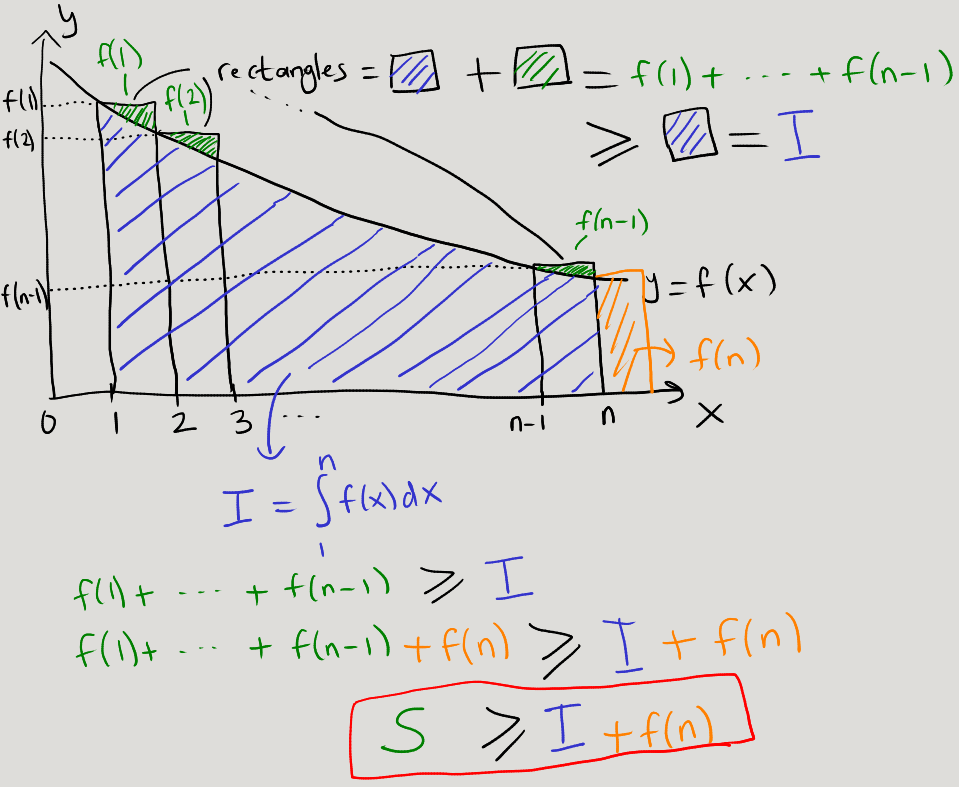
\includegraphics[scale=0.5]{integral-1.png}
\end{figure}
\begin{figure}[ht!]
\centering
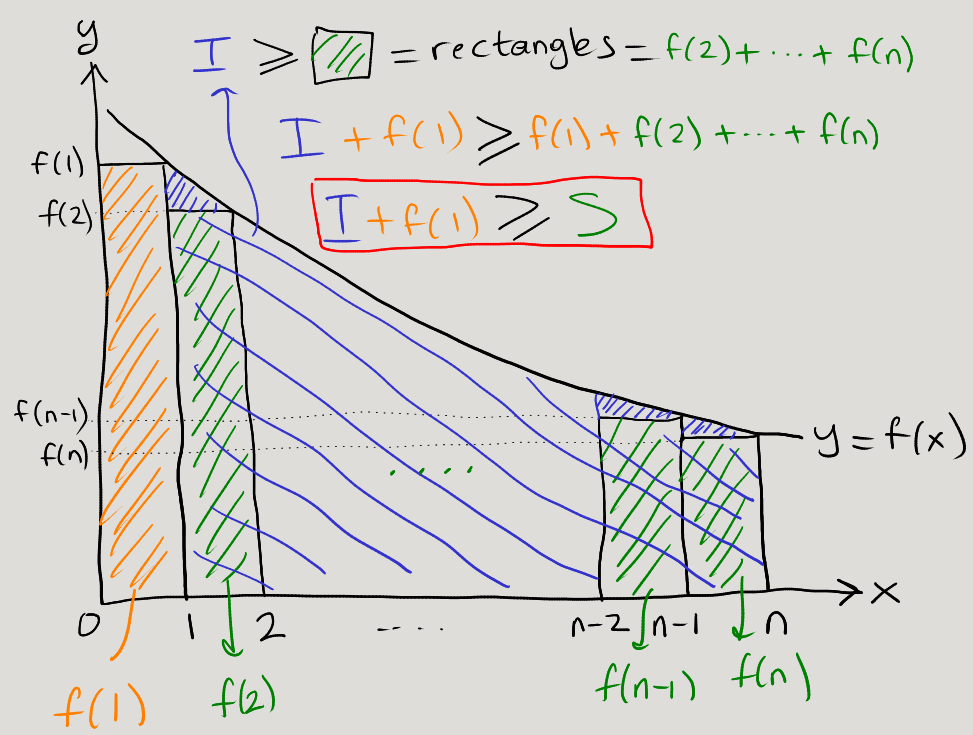
\includegraphics[scale=0.5]{integral-2.png}
\end{figure}
\end{proof}

\section{Problem 4}
Sammy the Shark is a financial service provider who offers loans on the following terms.

Sammy loans a client $m$ dollars in the morning. This puts the client $m$ dollars in debt to Sammy.

Each evening, Sammy first charges a service fee which increases the client’s debt by $f$ dollars, and then Sammy charges interest, which multiplies the debt by a factor of $p$. For example, Sammy might charge a “modest” ten cent service fee and 1\% interest rate per day, and then $f$ would be $0.1$ and $p$ would be $1.01$.

\subsection{(a)}
What is the client’s debt at the end of the first day?
\begin{proof}
At the end of day 1, debt increases from $m$ to $m+f$ then gets multiplied by a factor of $p$, so it's $p(m+f) = pm + pf$.
\end{proof}

\subsection{(b)}
What is the client’s debt at the end of the second day?
\begin{proof}
Again we increase debt from day 1 by $f$, then multiply this new debt by $p$, so it's: $p(pm + pf + f) = p^2m + p^2f + pf$.
\end{proof}

\subsection{(c)}
Write a formula for the client’s debt after $d$ days and find an equivalent closed form.
\begin{proof}
Before we attempt the closed formula let's see the third day debt:
$$
p(\text{2nd day debt} + f) = p(p^2m + p^2f + pf + f) = p^3m + p^3f + p^2f + pf
$$
The general formula after $d$ days seems to be: $p^dm + (p^df + p^{d-1}f + \ldots + p^2f + pf)$.

Writing this more nicely, we get:
$$
debt(d) = mp^d + fp(p^{d-1} + \ldots + 1) = mp^d + fp\,\frac{p^d-1}{p-1}
$$
We should prove this by induction. We are working with:
\begin{center}
$P(d) \Coloneqq$ the debt after $d$ days is: $\dps mp^d + fp\,\frac{p^d-1}{p-1}$.
\end{center}

{\bf Base Case.} $d = 1$. By part (a) the debt at the end of day 1 is $pm + pf$. And the formula gives:
$$
mp^1 + fp\,\frac{p^1-1}{p-1} = mp + fp
$$
which is the same. Therefore $P(1)$ is true.

{\bf Induction Step.} Assume $d \geq 1$ and assume $P(d)$ is true. Want to show $P(d+1)$.

By induction hypothesis the debt after $d$ days is
$$
mp^d + fp\,\frac{p^d-1}{p-1}
$$
At the end of day $d+1$ this increases by $f$ and gets multiplied by $p$. So the debt at the end of day $d+1$ is
$$
p(mp^d + fp\,\frac{p^d-1}{p-1} + f) = mp^{d+1} + fp\,\frac{p^{d+1}-p}{p-1} + fp
$$
If we factor out the $fp$ in the last two terms and get a common denominator, we get
$$
mp^{d+1} + fp(\frac{p^{d+1}-p}{p-1} + 1) = mp^{d+1} + fp(\frac{p^{d+1}-p}{p-1} + \frac{p-1}{p-1})
$$
Finally simplifying, we get
$$
mp^{d+1} + fp(\frac{p^{d+1}-p + p - 1}{p-1}) = mp^{d+1} + fp\,\frac{p^{d+1} - 1}{p-1}
$$
which proves $P(d+1)$. Therefore by Induction $P(d)$ is true for all $d \geq 1$.
\end{proof}

\subsection{(d)}
If you borrowed \$10 from Sammy for a year, how much would you owe him?
\begin{proof}
Here $m = 10, d = 365$ and we can use the values from the problem $f = 0.1, p = 1.01$ to get:
$$
10 \cdot 1.01^{365} + 0.1 \cdot 1.01 \cdot\frac{1.01^{365}-1}{1.01-1} = \$ 749.347030091
$$
\end{proof}

\section{Problem 5 (Supplemental problem)}
You’ve seen this neat trick for evaluating a geometric sum:
$$
\begin{array}{rcl}
S&=&1 + z + z^2 + \ldots + z^n\\
zS&=&z + z^2 + \ldots + z^n + z^{n+1}\\
S-zS&=&1-z^{n+1}\\
S&=&\dps\frac{1-z^{n+1}}{1-z}\\
\end{array}
$$
Use the same approach to find a closed form expression for this sum:
$$
T = 1z + 2z^2 + 3z^3 + \ldots + nz^n
$$

\begin{proof}
$$
\begin{array}{rcl}
T &=&1z + 2z^2 + 3z^3 + \ldots + (n-1)z^{n-1} + nz^n\\
zT&=&1z^2 + 2z^3 + \ldots + (n-1)z^n + nz^{n+1}\\
T-zT&=&z + z^2 + z^3 + \ldots + z^n + nz^{n+1}\\
T-zT+1&=&1 + z + z^2 + z^3 + \ldots + z^n + nz^{n+1}\\
T-zT+1 - nz^{n+1}&=&1 + z + z^2 + z^3 + \ldots + z^n\\
T-zT+1 - nz^{n+1}&=&S\\
T-zT+1 - nz^{n+1}&=&\dps\frac{1-z^{n+1}}{1-z}\\
T-zT&=&-1 + nz^{n+1} + \dps\frac{1-z^{n+1}}{1-z}\\
T(1-z)&=&-1 + nz^{n+1} + \dps\frac{1-z^{n+1}}{1-z}\\
T&=&\dps\frac{-1 + nz^{n+1}}{(1-z)} +\frac{1-z^{n+1}}{(1-z)^2}\\
\end{array}
$$
\end{proof}
\end{document}
